
Como etapa de pre-procesamiento, elegimos un pre-amplificador relativamente sencillo que implementa, control de volumen, selección de sensibilidad para tres fuentes de audio, \textbf{consumer} (cualquier fuente de un equipo comercial, como ser un celular), \textbf{línea} (fuente de valor standard como ser la salida de una placa de sonido) y \textbf{guitarra}, además el circuito implementa un control básico de tonos, con control de \textbf{Bass} y \textbf{Trebel}, con lo cual se tiene una llave selectora de tres puntos, un potenciómetro logarítmico para el volumen y dos potenciómetros lineales para el control de tonos. Para la implementación se necesitan tres amplificadores operacionales, para esta función seleccionamos el operacional \textbf{NE5532} de \textbf{Texas}, por su diseño específico para audio y su bajo ruido. El circuito es simple, la primer etapa es un atenuador conectado a la entrada de un amplificador no inversor, acoplado capacitivamente, la segunda etapa es un operacional con dos redes de realimentación para atenuar o graves alrededor de $100 \si[per-mode=symbol]{\hertz}$ o agudos alrededor de $10 \si[per-mode=symbol]{\kilo\hertz}$, el circuito original amplificaba, pero para adecuarlo a la sensibilidad de nuestro amplificador lo modificamos para que siempre la salida esté por debajo de $\si[per-mode=symbol]{1.1 \volt}$, para esto el circuito cuenta con una serie de presets en la etapa de salida que permiten ajustar el selector de sensibilidades y la ganancia global para adaptarse perfectamente a nuestro amplificador.


\vfill

\clearpage


\begin{figure}[H]
	\centering
	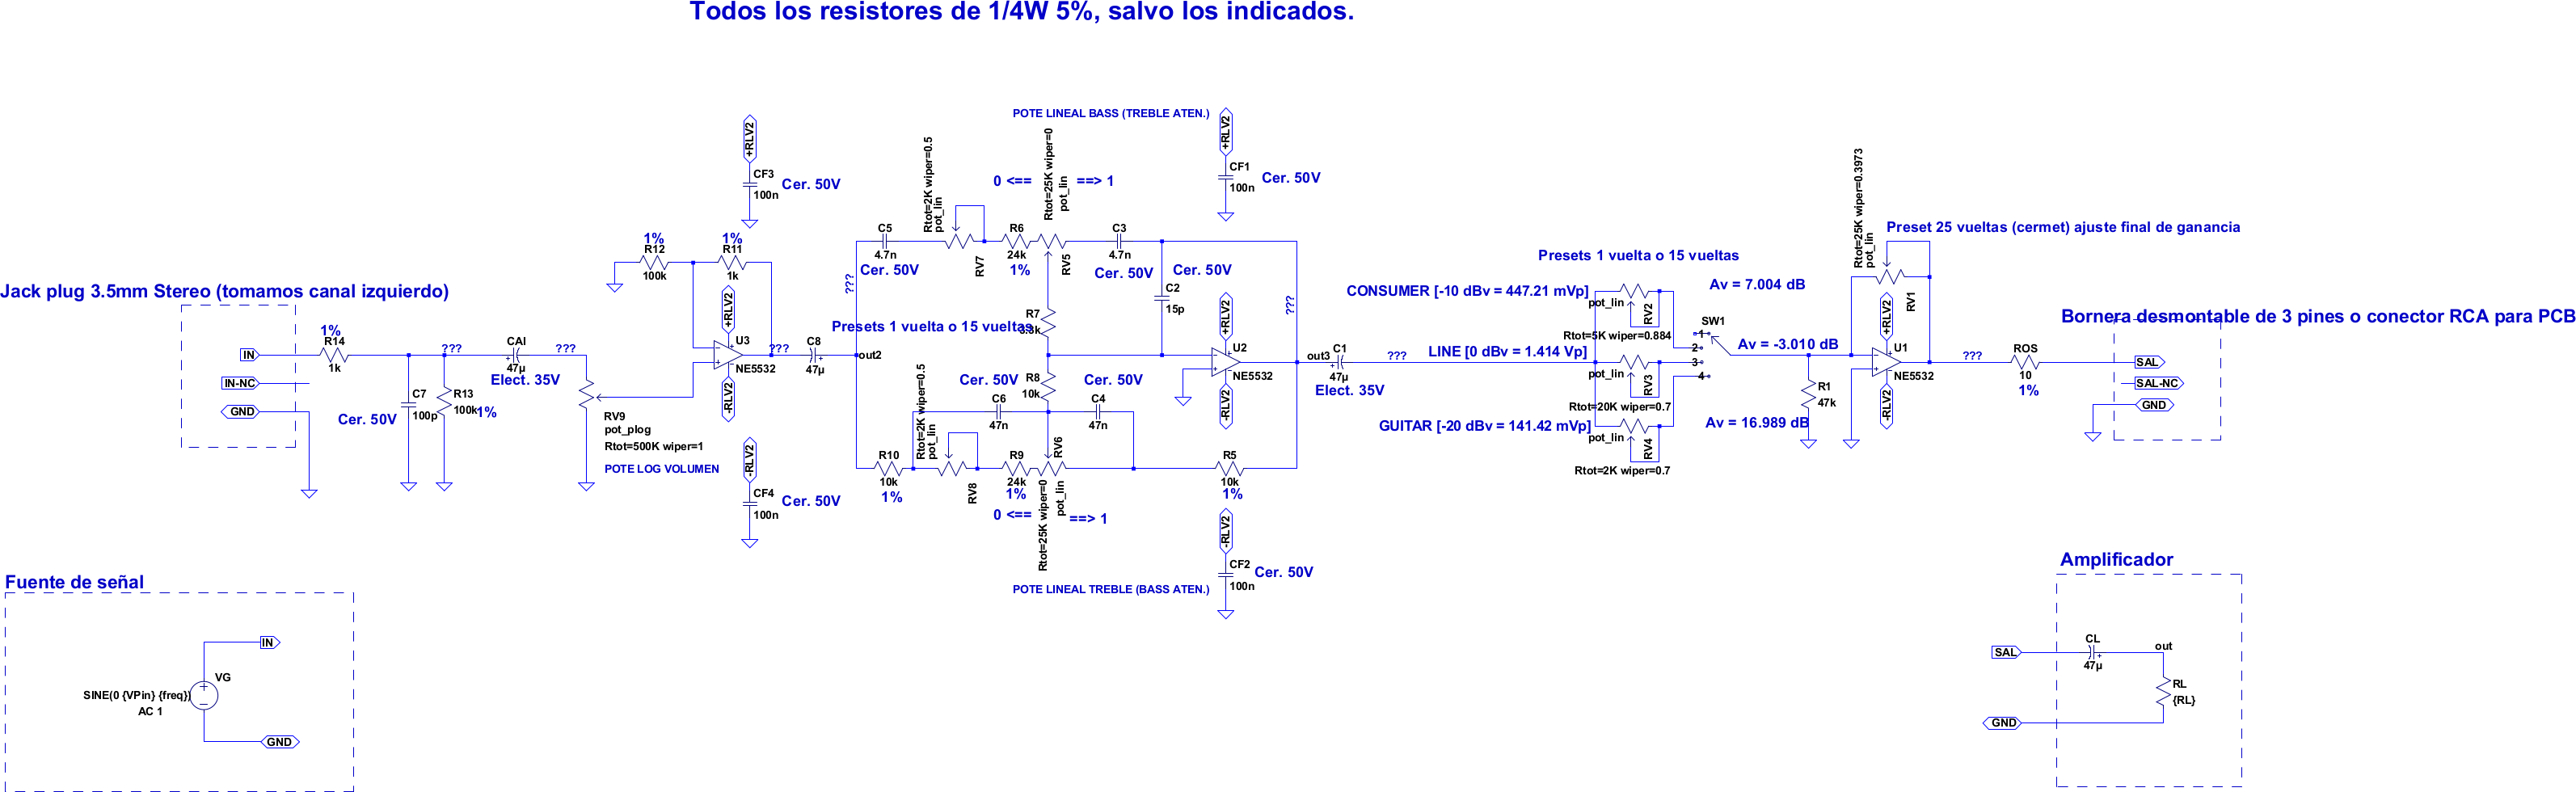
\includegraphics[width=0.7\paperheight, angle=90]{img/preamp.png}
	\caption{pre-amplificador con control de tonos y volumen.}
	\label{fig:power_supply}
\end{figure}